%%%%%%%%%%%%%%%%%%%%%%%%%%%%%%%%%%%%%%%%%%%%%%%%%%%%%%%%%%%%%%%%%%%%%%%%%%
% The template begins here. Please do not modify the font size from 12 point.

\documentclass[12pt]{article}
\usepackage{phase1}

%%%%%%%%%%%%%%%%%%%%%%%%%%%%%%%%%%%%%%%%%%%%%%%%%%%%%%%%%%%%%
%  PREAMBLE: sets up compiler modes, loads packages, defines macros, etc
%%%%%%%%%%%%%%%%%%%%%%%%%%%%%%%%%%%%%%%%%%%%%%%%%%%%%%%%%%%%%
%%%%%%%%%%%%%%%%%%%%%%%%%%%%%%%%%%%%%%%%%%%%%%%%%%%%%%%%%%%%%
%  PREAMBLE: sets up compiler modes, loads packages, defines macros, etc
%  Steve Rodney, 2012
%%%%%%%%%%%%%%%%%%%%%%%%%%%%%%%%%%%%%%%%%%%%%%%%%%%%%%%%%%%%%


%%%%%%%%%%%%%%%%%%%%
% COMPILER MODES
%%%%%%%%%%%%%%%%%%%%

% Changetext mode : highlight modified text in bold blue font
\newif{\ifchangetext}
\changetextfalse

%% Read in the -options.tex file (generated by the Makefile)
%%  to set the compile-mode options
\InputIfFileExists{\jobname-options}


%%%%%%%%%%%%%%%%%%%%%%%%%%%%%%%
% changetext  mode settings
%%%%%%%%%%%%%%%%%%%%%%%%%%%%%%%
\ifchangetext
  % Changed text is highlighted in bold, blue font 
  \newcommand{\change}[1]{\textcolor{blue}{ \bf #1}}
  \newcommand{\changenote}[1]{\textcolor{blue}{ \bf #1}}
\else
  % Changed text is indistinguishable
  \newcommand{\change}[1]{#1}
  \newcommand{\changenote}[1]{}
\fi


%%%%%%%%%%%%%%%%%%%%
% PACKAGES INCLUDED
%%%%%%%%%%%%%%%%%%%%
\usepackage{deluxetable}  % stand-alone version of AAStex's  deluxetable
\usepackage{journalnames} % Astro Journal abbreviations
\usepackage[svgnames]{xcolor}  % colored text (better than color)
%\usepackage[usenames]{color}  % colored text
\usepackage[linkcolor=blue,citecolor=darkgray,colorlinks=true]{hyperref}
\usepackage{natbib}   % reference citations and bibliography
\usepackage{graphicx}
%\usepackage{enumerate}% enumerated lists
\usepackage{amsmath}  % equations and such
\usepackage{amssymb}  % extended symbols lib
%\usepackage{mathrsfs} % extended math fonts (mathscr)
%\usepackage{breqn}    % automatic line breaks for long equations
%\usepackage{multirow}  % muti-row table cells
%\usepackage{paralist} % inline enumeration (for Table ref lists)
%\usepackage{authblk}
%\usepackage{multicol}
%\usepackage{subfig} % subfloats with independent captions
%\usepackage{subcaption} % subfloats with independent captions
\usepackage{setspace} % switch from double to single spacing
%\usepackage[none]{hyphenat} % Suppress the hyphenating
%\usepackage{verbatim} % verbatim text formatting
%\usepackage{ulem} % for some underlining.
%\usepackage{wrapfig}


%%%%%%%%%%%%%%%%%%%%%%%%%%%%%%%%%%%%%%%%%%%%%%%%%%%
% PDF mode settings : Auto-select eps or pdf figures 
% based  on the compiler used (i.e. latex vs pdflatex)
%%%%%%%%%%%%%%%%%%%%%%%%%%%%%%%%%%%%%%%%%%%%%%%%%%%
\DeclareGraphicsExtensions{.png,.pdf,.jpg}

%%%%%%%%%%%%%%%%%%%%%%%%%%%%%%%
% AUTHOR-DEFINED MACROS
%%%%%%%%%%%%%%%%%%%%%%%%%%%%%%%

% Time delay 
\def\dt{\ensuremath{\Delta t}}
\def\Dl{\ensuremath{D_l}}
\def\Ds{\ensuremath{D_s}}
\def\Dls{\ensuremath{D_{ls}}}

% plus-minus symbols for statistical or systematic errors
\def\pmstat{\ensuremath{\substack{\pm \\ \mbox{\scalebox{0.45}{stat}}}}}
\def\pmsys{\ensuremath{\substack{\pm \\ \mbox{\scalebox{0.45}{sys}}}}}


% prompt Ia fraction
\def\fp{\ensuremath{f_{P}}}
\def\fP{\ensuremath{f_{P}}}

% STARDUST probabilities
\def\pIa{\ensuremath{p_{Ia}}}
\def\pIaz{\ensuremath{p_{Ia,z}}}
\def\pIahost{\ensuremath{p_{Ia,host}}}

% General purpose usefulness:
\newcommand{\etal}{{et al.~}}                                             
\def\eg{{e.g.}}
\def\ie{{i.e.}}
\def\etc{{etc.}}
\newcommand{\lta}{\lesssim}                                               
\newcommand{\gta}{\gtrsim}                                                
\newcommand{\gt}{\gtsim}

% Cosmology:
\def\Om{\ensuremath{\Omega_{\rm m}}}
\def\Ot{\ensuremath{\Omega_{\rm tot}}}
\def\Ob{\ensuremath{\Omega_{\rm b}}}
\def\OL{\ensuremath{\Omega_{\Lambda}}}
\def\Ok{\ensuremath{\Omega_{\rm k}}}
\def\om{\ensuremath{\omega_{\rm m}}}
\def\ob{\ensuremath{\omega_{\rm b}}}
\def\wo{\ensuremath{w_0}}
\def\wa{\ensuremath{w_{\rm a}}}
\def\lcdm{$\Lambda$CDM}
\def\LCDM{$\Lambda$CDM}
\def\wcdm{$w$CDM}
\def\Ho{\ensuremath{H_0}}
\def\DA{\ensuremath{D_A}}
\def\DL{\ensuremath{D_L}}

% Astronomy:
\def\arcsec{\ensuremath{^{\prime\prime}}} 
\def\kms{\ensuremath{{\rm km s}^{-1}}}
\def\hgpcq{\mbox{$h^{-3}$Gpc$^3$}}
\def\hmpcq{\mbox{$h^{-3}$Mpc$^3$}}
\def\perhmpcq{\mbox{$h^{3}$Mpc$^{-3}$}}
\def\hmpc{\mbox{$h^{-1}$Mpc}}
\def\hmpci{\mbox{$h$\,Mpc$^{-1}$}}
\def\mpc{\mbox{Mpc}}
\def\mpci{\mbox{Mpc$^{-1}$}}
\def\mpcq{\mbox{Mpc$^{-3}$}}
\def\Msun{\mbox{M$_{\odot}$}}
\def\Av{\mbox{$A_V$}}
\def\Rv{\mbox{$R_V$}}

% Supernovae : 
\newcommand{\SNuVol}{\ensuremath{10^{-4}~\mbox{yr}^{-1}~\mbox{Mpc}^{-3}~{\mbox{h}_{70}}^{3}}}
\newcommand{\CCSN}{CC\,SN}
\newcommand{\CCSNe}{CC\,SN}
\newcommand{\TNSN}{TN\,SN}
\newcommand{\TNSNe}{TN\,SNe}
\newcommand{\SNIa}{SN\,Ia}
\newcommand{\SNeIa}{SN\,Ia}
\newcommand{\SNRz}{SNR($z$)}
\def\Mch{\mbox{M$_{\rm Ch}$}}
\def\Ni{\ensuremath{^{56}\mbox{Ni}}}
\newcommand{\dmfifteen}{\ensuremath{\Delta\mbox{m}_{15}}}
\newcommand{\deltamfifteen}{\ensuremath{\Delta\mbox{m}_{15}}}
\newcommand{\NM}{\ensuremath{\mbox{\rm N}_{Ia}/\mbox{M}_{*}}}

\def\galsnid{{\it galsnid}}

% SNANA / SALT2
\def\xone{\ensuremath{x_{1}}}
\def\C{\ensuremath{\mathcal{C}}}


% Missions:
\def\HST{{\it HST}}
\def\Hubble{{\it Hubble}}
\def\Hubbles{{\it Hubble's}}
\def\Spitzer{{\it Spitzer}}
\def\Chandra{{\it Chandra}}
\def\Herschel{{\it Herschel}}
\def\XMM{{\it XMM}}


%%%%%%%%%%%%%%%%%%%%%%%%%%%%%%%
% Page Setup 
%%%%%%%%%%%%%%%%%%%%%%%%%%%%%%%
\renewcommand{\topfraction}{0.9}
\renewcommand{\bottomfraction}{0.9}
\renewcommand{\textfraction}{0.1}
\renewcommand{\floatpagefraction}{0.9}
\renewcommand{\dbltopfraction}{0.9}
\renewcommand{\dblfloatpagefraction}{0.9}



%%%%%%%%%%%%%%%%%%%%%%%%%%%%%%%%%%%%
%% Figure placement shortcuts    
%%%%%%%%%%%%%%%%%%%%%%%%%%%%%%%%%%%%

\newcommand{\insertfigwide}[2] {
\begin{figure*}
\begin{center}
\resizebox{\textwidth}{!}{\includegraphics{{#1}}}
\caption{{#2}}
\end{center}
\end{figure*}
}

\newcommand{\insertfigdouble}[3] {
\begin{figure*}
\begin{center}
\resizebox{0.45\textwidth}{!}{\includegraphics{{#1}}}
\resizebox{0.45\textwidth}{!}{\includegraphics{{#2}}}
\figcaption{{#3}}
\end{center}
\end{figure*}
}

\newcommand{\insertfigquad}[5] {
\begin{figure*}
\begin{center}
\resizebox{0.48\textwidth}{!}{\includegraphics{{#1}}}
\resizebox{0.48\textwidth}{!}{\includegraphics{{#2}}}
\resizebox{0.48\textwidth}{!}{\includegraphics{{#3}}}
\resizebox{0.48\textwidth}{!}{\includegraphics{{#4}}}
\figcaption{{#5}}
\end{center}
\end{figure*}
}

\newcommand{\insertfig}[2] {
\begin{figure}
\begin{center}
\resizebox{\columnwidth}{!}{\includegraphics{{#1}}}
\figcaption{{#2}}
\end{center}
\end{figure}
}


\begin{document}

%   1. SCIENTIFIC JUSTIFICATION
%       (see Section 9.1 of the Call for Proposals)
%
%
\justification          % Do not delete this command.
% Enter your scientific justification here. 


The HST archive now holds a deep trove of WFC3-IR imaging on
strong-lensing galaxy clusters at redshifts $z\sim0.5$.  Many of these
clusters have dozens of multiply-imaged background galaxies at
redshifts $1\lesssim z \lesssim 6$, which have been used to produce
well-constrained models of the cluster lensing potential.  When a
supernova (SN) inevitably appears within one of these multiply-imaged
galaxies, it will of course be multiply-imaged itself. 
% {\bf \em With
% this snapshot program, we propose to use WFC3-IR to discover the first
% ever multiply-imaged SN behind a strong lensing galaxy cluster --
% setting a new gold standard for future gravitational lens time delay
% measurements.}
% With even just a single lensed SN
% time delay, we will constrain \Ho\ to better than 6\%
% precision, provide
% powerful new constraints on dark energy parameters, and deliver a unique test
% of systematic biases in other cosmological probes.  Along with the
% accompanying GO program for ToO follow-up, {\bf \em this IR snapshot
% survey will }
 {\bf \em With this snapshot survey, we propose to use WFC3-IR to
discover the first ever multiply-imaged SN behind a strong lensing
galaxy cluster.}  Along with the accompanying GO proposal for ToO
follow-up, {\bf \em this program will set a new gold standard for
future gravitational lens time delay measurements.}  With even just a
single lensed SN time delay, we will constrain \Ho\ to better than 6\%
precision, provide powerful new constraints on dark energy parameters,
and deliver a unique test of systematic biases in other cosmological
probes.


\medskip
\noindent {\bf Time Delay Cosmography}

\noindent As light from a distant source passes through a galaxy cluster,
strong gravitational lensing causes multiple images to appear to the
observer, separated by a time delay 

\vspace{-5mm}
\hspace{-1.4cm}
\begin{tabular}{p{7cm}r}
% \dt = \frac{\Dl \Ds}{\Dls} ( 1 + z_l ) \phi
{\begin{align}
%\begin{equation}\label{eq:dt}
 %  \dt = \frac{\Dl \Ds}{\Dls} ( 1 + z_l ) \phi
%\end{equation}
  \dt = \frac{(1+z_L)}{c}\frac{\Dl \Ds}{\,\Dls} \phi, \label{eq:dt} \\
\mbox{where}~~ \phi = \frac{1}{2}(\theta-\beta)^2 - \psi(\theta), \label{eq:phi}
\end{align}}
&
\hspace{0.7cm}
\raisebox{-30mm}{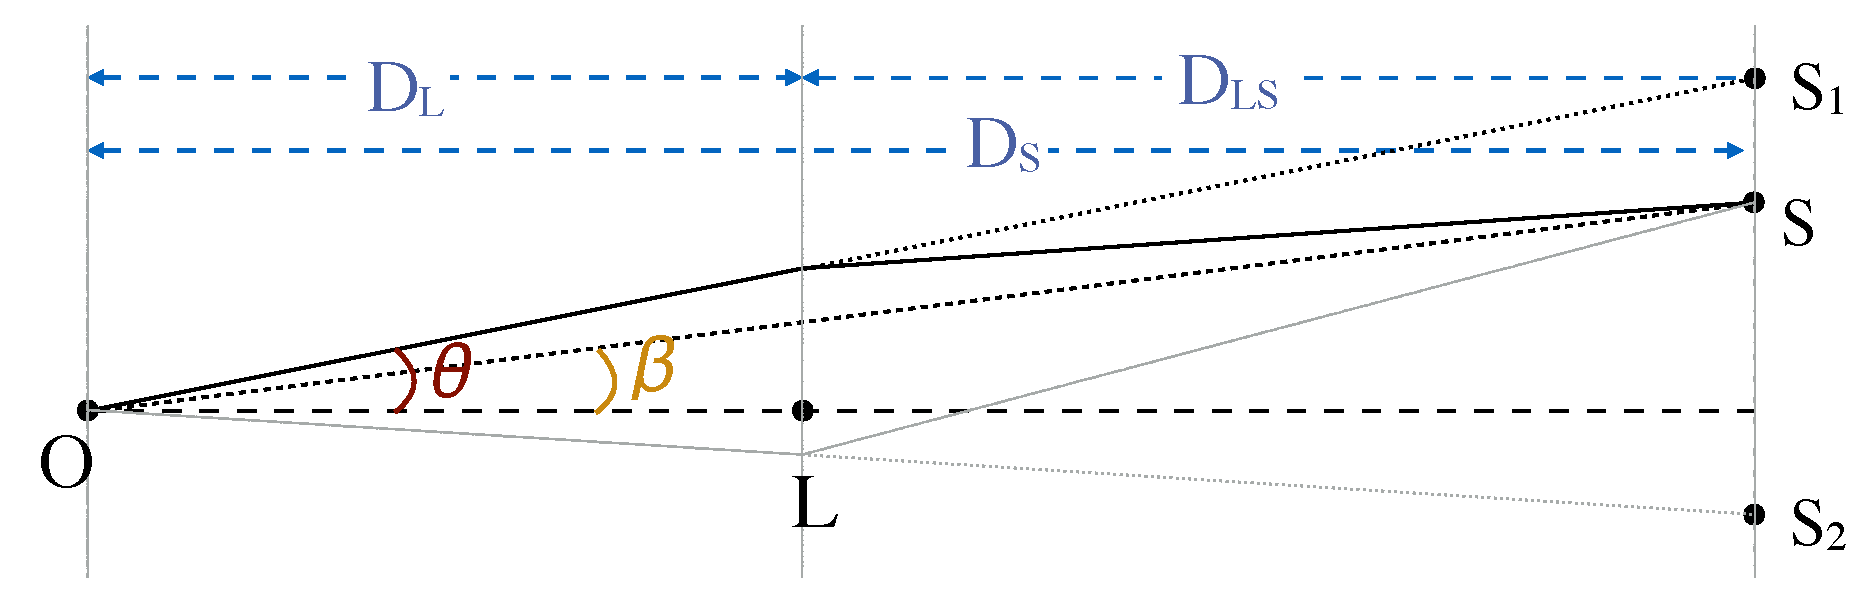
\includegraphics[width=0.52\textwidth]{../FIG/lensingGeometry2}}
\end{tabular}


\noindent and $z_L$ is the redshift of the lens, while \Dl, \Ds, 
and \Dls\ are angular diamater distances from the observer to the
lens, observer to source, and lens to source, respectively.  In
Eq.~\ref{eq:phi} for the time delay potential  ($\phi$), the first
term gives the geometric delay due to light rays following different
path lengths to the observer, and the second term, $\psi$, is the
relativistic component due to differing values of the gravitational
potential along each path.

The distance ratio $\Dl\Ds/\Dls$ in Equation~\ref{eq:dt} is known as
the {\em time delay distance}, and it carries a factor
of \Ho$^{-1}$. Thus, if the lensing potential $\phi$ is well known,
then a time delay measurement provides a direct measurement of the
Hubble constant -- independent of the local distance ladder.  The
distance ratio also has unusual sensitivities to cosmological
parameters as a function of redshift that make this technique a
particularly useful probe of dynamic dark energy
models \citep{Linder:2011}.

\citet{Refsdal:1964} first proposed the use of SN time delays as 
a means to measure \Ho.  Now 50 years later, this has not yet been
achieved, primarily due to the small number of very well analyzed
gravitational lenses ($\sim$dozens), and the short visibility window
for any given high-$z$ SN event ($\sim$a few weeks).  Only recently
have we begun to realize the potential in this technique, with the
measurement of a few dozen time delays of quasars, being lensed
typically by a single foreground galaxy \citep{Jackson:2007}. Among
these, only a handful have time delays measured with particularly high
precision \citep[e.g.][]{Suyu:2010,Suyu:2013}.  These quasar lenses
generally suffer from a number of serious concerns, notably: (1) the
lensing potential is poorly constrained due to inherent degeneracies
and insufficient constraints; (2) the time delays and angular
separations are quite small (tens of days, fractions of an arcsecond);
and (3) the source is stochastically variable, often requiring years of
stable monitoring for the time delay measurement.  Wide-field surveys
in the coming decade could deliver $>$100 quasar time delays, but
these problems represent unavoidable systematic biases for this
sample.

\medskip
\noindent {\bf The SN Time Delay Advantage}
 
In Cycle 22, HST has just achieved a new capability for the discovery
of a strongly-lensed SN. The first key advancement was the
availability of WFC3-IR, which allows HST imaging surveys to capture
high-$z$ SN at the peak of their SED profile in rest-frame optical
bands \citep{Rodney:2012,Jones:2013}.  Ground-based surveys and even
HST/ACS programs have searched for multiply-imaged SN in the past, but
none have had the capability to detect even highly magnified SN at
$z>2$ \citep[e.g.][]{Dawson:2009,Sharon:2010,Sand:2011}.  With
WFC3-IR, \Hubble\ now has access to a much larger survey volume with
each pointing.

A WFC3-IR program targeting massive clusters, such as CLASH or the
Hubble Frontier Fields, could in principal have caught a strongly
lensed SN already.  CLASH, for example, collected
WFC3-IR imaging of 25 clusters over 3 years, but the time separation
between the first and last IR image on any single cluster was
typically only $\sim$40 days, so in practice each cluster only had one
epoch suitable for a lensed SN search. 
However, CLASH and other programs have now provided the second critical
advance: deep IR template imaging of massive clusters from which to
construct difference images for SN discovery.  These HST programs have
also led to an explosion of detailed mass modeling for strong-lensing
clusters, % providing well-defined lensing potentials that will be
which is crucial for evaluating a multiply-imaged SN when one is found.

Our snapshot program will capitalize on this rich new treasury,
%in the
%HST archive, opening the door for a pioneering time delay distance
%measurement with the discovery of one or more strongly lensed SN
%behind a galaxy cluster.  We will 
focusing on well-studied massive clusters
that act as especially strong lenses (Table~\ref{tab:clusters}). For
each of these clusters we have dozens of known multiply-imaged
galaxies, and we already have state-of-the-art lens models in
hand \citep[e.g.][]{Zitrin:2011a,Zitrin:2011b,Zitrin:2012a,Zitrin:2012b,Zitrin:2013}.
Wherever a multiply-imaged SN should appear, {\bf \em we will be
starting out with much better constraints on the lensing potential
$\phi$} than are available for most quasar time-delay lenses. 
%In
%addition to improving the quality of the time-delay cosmography, this
%fore-knowledge of the lensing potential will also be crucial for
%quickly evaluating any lensed SN candidates we discover, to weed out
%impostors before investing precious follow-up time.

Furthermore, {\bf \em the SN we discover behind these clusters will be
inherently better time-delay sources} than the existing sample of
quasars.  Typical time delays through our target clusters are months
or years (not days or weeks as for many lensed quasars), allowing for
more precise measurements of \dt, with ample time to prepare for the
appearance of the second image.  Also, the SN light curve has a single
peak, so there is no possibility of phase ambiguity, and the age of a
SN relative to explosion can be precisely defined from light curve
shape and color, or from spectroscopic
cross-correlation \citep{Filippenko:1997,Blondin:2007}.  Thus the time
delay measurement does not require continuous long-term monitoring,
and can be made with minimal systematic uncertainties.  Finally, if
the SN is of Type Ia (a likely prospect), then light curve fitting can
provide a luminosity distance measurement with $\sim$8\%
precision \citep{Phillips:1993}, and this lensed \SNIa\ could easily
be among the most distant \SNIa\ ever seen.
% Galaxy cluster distances can also be
% estimated using the Sunyaev-Zeldovich effect and x-ray cluster
% luminosities \citep{Silk:1978}.  This means that in addition to the
% time delay distance ratio (\Dl\Ds/\Dls) we can also measure
% independent distances to both the lens and the source.  A \SNIa\ that
% is multiply-imaged by a galaxy cluster would therefore provide a
% unique chance to test for systematic biases in these distance
% estimators.
% %, or even to perform the distance-duality test: if the
% %ratio $\eta_{DD} = D_{S}^{(L)} / ( D_{S}^{(A)}(1+z_S)^2 )$ deviates
% %from unity, then this would signal systematic errors in one or more
% %distances, or a fundamental flaw in the concordance cosmology.


% The large angular separations between our lensed sources and their
% unlensed sight-lines will allow for very precise astrometry that is
% free of systematics due to source blending.  



\medskip
\noindent {\bf The HST Snapshot Search Strategy }

%Since Cycle 17, HST surveys of strong lensing clusters (notably CLASH
%and the Frontier Fields) have been investing hundreds of orbits in deep
%WFC3-IR imaging.  With these templates in hand, the most efficient
%way to discover a strongly lensed SN is through a relatively
%small snapshot program.    
To estimate the number of snapshots we need, we start with a
tabulation of the number of known multiply-imaged galaxies in the
fields of our target clusters (Table~\ref{tab:clusters}).  This is a
conservative approach, as it is quite possible to detect a
multiply-imaged SN even if the host galaxy is well below the current
detection thresholds for these cluster fields. The total yield of
strongly-lensed SN per snapshot is 
$N_{SN} = SNR_{M} \times M_{gal} \times N_{gal} \times t_{vis}$. 
Here $SNR_M$ is the SN rate per unit mass, $M_{gal}$ is
the average mass of a multiply-imaged galaxy, $N_{gal}$ is the number
of multiply imaged galaxies in the field, and $t_{vis}$ is the length
of time that any given SN is visible to our snapshot survey.  

Most of the lensed systems in our target list are at $z\sim 2$, in an
era near the peak of the cosmic star formation history, so we assume
that our average lensed galaxy is generating SN at a rate similar to
an Sc galaxy in our local universe: $SNR_{M} \sim0.2
(100 \mbox{yr})^{-1} (10^{10} \Msun)^{-1}$ for \SNIa\ and $0.7
(100 \mbox{yr})^{-1} (10^{10} \Msun)^{-1}$ for Type
II \citep{Mannucci:2005}.  We adopt an average stellar mass of
$M_{gal}=10^{10.7} \Msun$ \citep{Tomczak:2013}, and use the census of
multiply-imaged systems in Table~\ref{tab:clusters} to predict an
average of $N_{gal}\sim 35$ lensed galaxy images per
cluster.\footnote{Note that we count each separate image of a
multiple-image set except the last one (we can't measure a time delay
from the last appearance). The time delay between each image is of
order months or years, so each snapshot is essentially observing the
same galaxy at several widely-spaced epochs that can be treated as
independent.}  Using simulated SN light curves in 240 multiply-imaged
galaxies (Figure~\ref{fig:tvis}), we find an average $t_{vis}\sim 30$
days for \SNIa\ and $\sim$20 days for SN II.


With these relatively conservative estimates, we estimate $N_{SN}\sim
0.1$ SN per snapshot, including both Type Ia and II.  To give this
program a good chance at discovering a strongly lensed SN in Cycle 22,
we request 200 snapshots.  Assuming a realistic snapshot execution
rate of $\sim$30\%, this program should yield a sample of $\sim 6 \pm
4$ SN in one year.  Even if our yield prediction is biased high by a
factor of $\sim$2, we still have a better than 68\% chance to catch at
least one.  Given the intrinsic value of each lensed SN, even just a
single detection will nevertheless be an extraordinary step forward
for time delay cosmography.

Finally, we note that this snapshot program is designed only for
discovery. Follow-up observations will come from accompanying GO
program, using 12 orbits with ToO observations for immediate
confirmation of a SN candidate and measurement of the light curve.
Sometime in the future, a return campaign to catch the next image
would be needed to complete the time delay measurement, using HST,
ground-based AO systems, or possibly JWST, depending on the length of
the delay.


% \medskip
% \noindent{\bf Lensed \SNIa\ Probing Cluster Models} 
% We could find lensed SN Ia with significant magnification that do not
% have multiple images, adding to the sample of SN lensing probes
% (Patel+ 2014, Nordin+ 2014).  Classification and light curve
% measurement could be done with FrontierSN follow-up orbits


%\insertfig{FIG/lightcurves.pdf}{ \label{fig:lightcurves} Lensed SN
%    light curves }







%%%%%%%%%%%%%%%%%%%%%%%%%%%%%%%%%%%%%%%%%%%%%%%%%%%%%%%%%%%%%%%%%%%%%%%%%%%

%   2. DESCRIPTION OF THE OBSERVATIONS
%       (see Section 9.2 of the Call for Proposals)
%
%
\describeobservations   % Do not delete this command.
% Enter your observing description here.
%\begin{wrapfigure}{r}{0.3\textwidth}
%\minipage[r]{0.29\textwidth}
%   
\begin{wraptable}{r}{2.25in}
 \caption{Detection Limits \label{tab:detectionLimits}}
 \begin{tabular}{ccc}
  \toprule
  \toprule
   WFC3/IR & Exp.Time & m$_{lim}$ $^{*}$ \\
   Filter  &  [min] &  [AB mag] \\
   \midrule
   F110W   &    12  &   26.3 \\
   F110W   &    20  &   26.6 \\
   F110W   &    30  &   26.9 \\
   F140W   &    12  &   25.9 \\
   F140W   &    20  &   26.2 \\ 
   F140W   &    30  &   26.5 \\
  \bottomrule
 \multicolumn{3}{p{2.6in}}{$^*$\,Apparent magnitude that yields S/N of 5 (optimum S/N$\sim$10) in the given exposure time.}
\end{tabular}
\end{wraptable}




%\end{minipage}
%\end{wrapfigure}


%%%%%%%%%%%%%%%%%%%%%%%%%%%%%%%%%%%%%%%%%%%%%%%%%%%%%%%%%%%%%%%%%%%%%%%%%%%

%   3. SPECIAL REQUIREMENTS
%       (see Section 9.3 of the Call for Proposals)
%
%
\specialreq             % Do not delete this command.
% Justify your special requirements here, if any.
\input{specialreqGO}

%%%%%%%%%%%%%%%%%%%%%%%%%%%%%%%%%%%%%%%%%%%%%%%%%%%%%%%%%%%%%%%%%%%%%%%%%%%

%   4. COORDINATED OBSERVATIONS
%       (see Section 9.4 of the Call for Proposals)
%
%
%\coordinatedobs          % Do not delete this command.
% Enter your coordinated observing plans here, if any.
%\input{coordinatedobsGO}

%%%%%%%%%%%%%%%%%%%%%%%%%%%%%%%%%%%%%%%%%%%%%%%%%%%%%%%%%%%%%%%%%%%%%%%%%%%

%   5. JUSTIFY DUPLICATIONS
%       (see Section 9.5 of the Call for Proposals)
%
%
\duplications           % Do not delete this command.
% Enter your duplication justifications here, if any.
\input{duplicationsGO}


%%%%%%%%%%%%%%%%%%%%%%%%%%%%%%%%%%%%%%%%%%%%%%%%%%%%%%%%%%%%%%%%%%%%%%%%%%%
%  Bibliography goes in before or after PAST HST usage ??
%  Probably before, since it has to be counted in the text page limit
%%%%%%%%%%%%%%%%%%%%%%%%%%%%%%%%%%%%%%%%%%%%%%%%%%%%%%%%%%%%%%%%%%%%%%%%%%%

%\smallskip
\newpage
\setlength{\bibsep}{-2pt}
\begin{spacing}{0.5}
\bibliographystyle{apjbrief}
{\footnotesize
\bibliography{bibdesk}
}
\end{spacing}



%%%%%%%%%%%%%%%%%%%%%%%%%%%%%%%%%%%%%%%%%%%%%%%%%%%%%%%%%%%%%%%%%%%%%%%%%%%

%   7. FIGURES AND TABLES  (must appear after the text)
\input{figuresGO}


%%%%%%%%%%%%%%%%%%%%%%%%%%%%%%%%%%%%%%%%%%%%%%%%%%%%%%%%%%%%%%%%%%%%%%%%%%%

%   6. PAST HST USAGE
%       (see Section 9.8 of the Call for Proposals)
%
%        List here the program numbers and data status for all accepted GO/AR/SNAP 
%        programs of the PI in at least the last four HST Cycles. Include a list of refereed publications 
%        resulting from these programs.       
%
%       Note that the description of past HST usage  DOES NOT count against the page limits of the proposal.
%

%\pagebreak
\newpage
\pasthstusage  % Do not delete this command.

% all accepted GO/AR/SNAP Programs of the PI in the last four HST cycles.

Table\,\ref{tab:pasthstusage} lists the HST programs from recent cycles that include PI Rodney.

% \begin{deluxetable}{p{0.25\linewidth}p{0.15\linewidth}p{0.2\linewidth}p{0.3\linewidth}}
% %\rotate
% \tablecolumns{4}
% \tablecaption{Past HST Usage for PI \label{tab:pasthstusage}}
% \tablehead{   \colhead{PID}  & \colhead{Title} & \colhead{Status} & 
%   \colhead{Selected Publications\tablenotemark{*}} }
% \startdata
% 12060-64, 12440-45 & CANDELS & Cycle 18-20 MCT;\linebreak $\sim$90\% complete. & \citealt{Grogin:2011}\linebreak \citealt{Trump:2011}\linebreak \citealt{van-der-Wel:2011} \\[6pt]
% 12065-69, 12100-04, 12451-60 & CLASH & Cycle 18-20 MCT;\linebreak $\sim$90\% complete. & \citealt{Postman:2012}\linebreak \citealt{Coe:2013}\\[22pt]
% 12099, 12461, 13063 & C+C SN Follow-up & Cycle 18-20 MCT;\linebreak $\sim$90\% complete. & \citealt{Rodney:2012}\linebreak \citealt{Frederiksen:2012}\linebreak \citealp{Jones:2013}\\[6pt]
% 13046 & RAISIN & Cycle 20 ToO;\linebreak collecting data & \nodata \\
% \enddata
% \tablenotetext{*}{Listed publications are those with direct input from PI Rodney and the CANDELS+CLASH SN team. Total CANDELS+CLASH publications $\approx$63.}
% \end{deluxetable}






\end{document}          % End of proposal. Do not delete this line.
                        % Everything after this command is ignored.

